\documentclass[11pt]{article}

% --- Packages (all standard; auto-fetched by tectonic, present in any full TeX Live) ---
\usepackage{amsmath}
\usepackage{amssymb}
\usepackage{booktabs}
\usepackage{tabularx}
\usepackage{longtable}
\usepackage[margin=1in]{geometry}
\usepackage{graphicx}
\usepackage{float}     % provides [H] for exact figure placement
\usepackage{parskip}
\usepackage{xcolor}
\definecolor{linknavy}{HTML}{1A5276}
\usepackage{tocloft}   % styles the 'Topics covered' contents list (load before hyperref)
\usepackage{hyperref}  % load last; provides \url and makes the ToC clickable
\hypersetup{
  colorlinks=true,
  linkcolor=linknavy,   % internal links (Topics-covered ToC entries)
  urlcolor=linknavy,     % DOIs in the reference list
  citecolor=linknavy,
  bookmarksnumbered=true,
  pdftitle={Supplementary Methods}
}

% --- 'Topics covered' contents list: professional ruled layout (tocloft) ---
\renewcommand{\cfttoctitlefont}{\large\bfseries}                       % heading font
\renewcommand{\cftaftertoctitle}{\par\vspace{2pt}\hrule height 0.4pt\vspace{5pt}} % rule under heading
\setlength{\cftbeforetoctitleskip}{2pt}
\setlength{\cftaftertoctitleskip}{0pt}
\renewcommand{\cftsecfont}{\normalsize}                                % entry title
\renewcommand{\cftsecpagefont}{\normalsize}                            % page number
\renewcommand{\cftsecaftersnum}{.}                                     % "1." not "1"
\renewcommand{\cftsecleader}{\normalfont\cftdotfill{\cftdotsep}}       % dotted leaders
\setlength{\cftsecnumwidth}{2.0em}                                     % number column width
\setlength{\cftbeforesecskip}{3pt}                                     % gap between entries

% Ragged-right wrapping X column for the tables
\newcolumntype{Y}{>{\raggedright\arraybackslash}X}

\title{\vspace{-2.0em}\textbf{Supplementary Methods}\\[0.35em]
\large One-dimensional stochastic modelling of loop extrusion, transcription
and nucleotide-excision repair}
\date{}
\author{}

\begin{document}
\maketitle
\vspace{-1.0em}

% --- Topic specification (built from the \section headings); styling in preamble ---
\begingroup
\setlength{\parskip}{0pt}
\renewcommand{\contentsname}{Topics covered}
\noindent\rule{\linewidth}{0.8pt}\par\nobreak
\tableofcontents
\nobreak\vspace{3pt}
\noindent\rule{\linewidth}{0.8pt}
\endgroup
\bigskip

% =====================================================================
\section{Model overview, time steps and lattice setup}

We modelled interphase chromatin as a one-dimensional lattice and simulated the
stochastic dynamics of three agent species along it: cohesin loop-extrusion
complexes, RNA polymerase II, and ultraviolet photolesions. Building on
established stochastic lattice models of loop extrusion (Fudenberg et al., 2016;
Banigan et al., 2020) and the polychrom simulation framework (Imakaev et al., 2019), the system advanced in discrete, fixed-length time steps; within each
step we updated lesion states, then (when transcription was active) recruited and
translocated polymerases, and finally translocated cohesin, under hard occupancy
exclusion so that no two agents shared a site. State transitions (binding,
dissociation, stage changes, capture and release) were memoryless, each drawn as
a per-step Bernoulli trial equivalent to a first-order (Poisson) process; we report
each as a rate constant or its characteristic time. We did not simulate the
three-dimensional polymer. The features that population contact maps and single-locus
imaging are most sensitive to (the one-dimensional cohesin distribution, the spans of
the loops it extrudes, and the sites where extrusion is impeded) are themselves
one-dimensional, and can be sampled with far greater statistical depth this way.

Two identities fixed the physical scale. Each lattice site corresponded to 250~bp of
DNA, and each time step corresponded to 2~s of real time. All velocities,
lifetimes and rates are reported in physical units after applying these
identities. Each memoryless transition fired with a per-step probability set by its
mean waiting time $\tau$,
%
\begin{equation}
p \;=\; \frac{\Delta t}{\tau} \;\approx\; 1 - e^{-\Delta t/\tau},
\qquad \Delta t = 2\ \mathrm{s},\ \ \ell = 250\ \mathrm{bp},
\end{equation}
%
so we report every such process by its characteristic time $\tau$ or equivalent
rate $1/\tau$. Magnitudes are tick-independent biology: a process is authored as a
rate or duration and converted to its per-step probability through Eq.~1, so the
same physical kinetics are recovered at any chosen step size. Kinetic constants
baked into the configuration use the exact form $1-e^{-\Delta t/\tau}$, while the
geometric per-step transitions evaluated inside the engine (cohesin unbinding,
lesion recognition and repair) use the equivalent linear form $\Delta t/\tau$
(capped at one); the two agree to better than $0.1\%$ at the calibrated $\tau$. The
calibrated quantities are collected in Table~1.

We simulated a 10-Mb locus (40{,}000 sites) instantiated as twenty independent
replicate copies (200~Mb of lattice in total), equilibrated each replicate for
$\approx$22~h of simulated time (40{,}000 steps), and then sampled an
$\approx$89~h production trajectory (160{,}000 steps). The configurations and
analyses are described in Section~8.

\medskip
\noindent\textbf{Table 1. Calibrated model parameters.} Values are reported in
physical units after applying the lattice (1 site $=$ 250~bp) and temporal
(1 step $=$ 2~s) calibrations.

\medskip
\setlength{\LTleft}{0pt}\setlength{\LTright}{\fill}
\begin{longtable}{@{}>{\raggedright\arraybackslash}p{3.7cm} >{\raggedright\arraybackslash}p{3.4cm} >{\raggedright\arraybackslash}p{7.3cm}@{}}
\toprule
Parameter & Calibrated value & Basis \\
\midrule
\endfirsthead
\toprule
Parameter & Calibrated value & Basis \\
\midrule
\endhead
\bottomrule
\endlastfoot
\multicolumn{3}{@{}l}{\textit{System}}\\
Spatial resolution & 250~bp per site & calibration \\
Temporal resolution & 2~s per step & calibration \\
Simulated locus & 10~Mb $\times$ 20 replicates (200~Mb) & --- \\
Equilibration / production & $\approx$22~h / $\approx$89~h & --- \\
\addlinespace
\multicolumn{3}{@{}l}{\textit{Loop extrusion}}\\
Cohesin separation (density) & one complex per 240~kb & Gabriele et al., 2022 \\
Subunit velocity & 125~bp\,s$^{-1}$ (7.5~kb\,min$^{-1}$) & see \S3 \\
Loop-extrusion rate & 250~bp\,s$^{-1}$ (15~kb\,min$^{-1}$) & $\approx$2$\times$ the in-vivo rate inferred for Gabriele et al., 2022 ($\approx$150~kb\,/\,$\approx$20~min; \S3); below in-vitro $\approx$0.5--2~kb\,s$^{-1}$ (Kim et al., 2019; Davidson et al., 2019) \\
Residence, free & $\approx$22.5~min & $\approx$22~min residence (Hansen et al., 2017); $\approx$20~min base lifetime (Gabriele et al., 2022) \\
Residence, CTCF-captured & $\approx$90~min ($\approx$4$\times$) & Gabriele et al., 2022 (stabilised fourfold) \\
Processivity (emergent) & a few $\times\,10^{2}$~kb & cf.\ $\approx$150~kb (Gabriele et al., 2022); 300~kb (Yang \& Hansen, 2024) \\
Recruitment & uniform & Banigan et al., 2023 \\
\addlinespace
\multicolumn{3}{@{}l}{\textit{Transcription}}\\
Promoter-proximal pause & $\approx$250~bp downstream & --- \\
Single-Pol pause (median / active) & $\approx$42~s / $\approx$25~s & $\approx$42~s mean live-cell residence (Steurer et al., 2018); $\approx$1.2--1.4~min model half-life (Zhao et al., 2023); multi-minute by decay-rate (Jonkers et al., 2014; Core \& Adelman, 2019) \\
Productive fraction (median; activity-graded) & $\approx$0.29 (range $\approx$0.14--0.47) & $\approx$0.2 ($\approx$80\% premature termination), STL-seq (Zimmer et al., 2021) \\
Initiation / loading, expressed (realised) & median $\approx$0.27~min$^{-1}$ (occupied genes); $\approx$0.05 all-gene & low $\approx$0.2 / high $\approx$1.0~min$^{-1}$ (Zhao et al., 2023); pause-initiation limit (Gressel et al., 2019) \\
Productive output, 3$'$ (realised) & detected median $\approx$0.02~min$^{-1}$/allele; active $\approx$0.1 & $\approx$2~mRNA\,h$^{-1}$ per gene (Schwanh\"ausser et al., 2011); $\approx$87~min$^{-1}$ for heat-shocked HSPA1A (Gressel et al., 2019) \\
Elongation velocity & 2.1~kb\,min$^{-1}$ (0.035~kb\,s$^{-1}$); $\approx$1.9 realised & in-vivo 1.3--4.3~kb\,min$^{-1}$ (Guo \& Price, 2013); 0.5--4 genome-wide (Jonkers et al., 2014); $\approx$2 assumed by Zhao et al., 2023 \\
3$'$ termination dwell & $\approx$1.8~min (realised) & derived (Fong et al., 2015; Cortazar et al., 2019) \\
\addlinespace
\multicolumn{3}{@{}l}{\textit{RNA Pol II -- cohesin}}\\
Cohesin transit past engaged Pol II & $\approx$100~s ($k \approx 0.01$~s$^{-1}$) & Banigan et al., 2023 \\
Cohesin transit past pre-initiation Pol II & $\approx$12~s ($\approx$8$\times$ more permeable) & --- \\
Subunit : elongation velocity ratio & $\approx$3.6 (loop $\approx$7) & Banigan et al., 2023 ($\ge$3--5) \\
\addlinespace
\multicolumn{3}{@{}l}{\textit{Lesions and repair}}\\
Lesion density (swept) & 1 per 7--100~kb (20~J\,m$^{-2}$; repair time-course, Table~2) & \S6 \\
TC-NER (Type A) fraction of gene-body lesions & $\le 0.5$ (ceiling); $\approx$0.20 (typical) & --- \\
Pre-repair stage & $\approx$40~min & --- \\
Active repair stage & $\approx$6~min & --- \\
Per-step block, repair stage & $\approx$0.993 (bypass $\approx$0.007 / step) & --- \\
\end{longtable}

% =====================================================================
\section{Topology: genes, domains and boundaries}

We generated the genomic substrate procedurally to reproduce the marginal
statistics of a gene-rich human locus. A smooth latent gene-density profile was
sampled along the locus and used to partition it into topologically associating
domains (TADs) whose lengths were anticorrelated with local gene density: dense
regions were tiled by shorter domains (target median $\approx$0.75~Mb) and sparse
regions by longer ones (target median $\approx$1.25~Mb), with individual lengths
drawn from a heavy-tailed distribution and bounded to $\approx$0.3--2.8~Mb,
bracketing the sub-megabase domain-size distribution of mammalian genomes (median
$\approx$0.88~Mb in mouse ES cells; Dixon et al., 2012). We scaled domains above the characteristic single-loop reach so that the
emergent observable was domain-level insulation rather than isolated loop
corner-peaks.

Each domain boundary was a permeable, oriented CTCF proxy with a per-encounter
probability of arresting an incident cohesin subunit, equivalent to CTCF occupancy.
Boundaries were oriented convergently (the left boundary arrested left-travelling
subunits and the right boundary right-travelling subunits), recapitulating the
inward CTCF-motif polarity required for stable looping. Arrest probabilities were
modest (tens of percent) and were set higher at boundaries flanking shorter, denser,
more transcriptionally active domains. Each boundary's strength was an equal-weight
blend of two drivers, the transcriptional activity and the gene density of its
flanking domains, each taken from the more extreme (more active, denser) of the two
flanks, so that boundary strength fell with domain length and active, gene-dense
domains were well insulated on both sides. The
two ends of the locus were reflecting.

We placed genes at a locus-average density of $\approx$12 per~Mb (122 genes across
the 10-Mb locus), with the
per-domain count following the same gene-density latent that set the domain
partition (so shorter, denser domains were more gene-dense), and with lengths
drawn from a log-normal distribution (median $\approx$23~kb) with a tail beyond
100~kb, matching the human gene-length distribution. Placement was non-overlapping
and interior genes were assigned transcriptional polarity at random, yielding
co-directional, convergent and divergent neighbours in their natural proportions.
Genes belonged to four regulatory classes: constitutive housekeeping, highly
expressed housekeeping, cell-type-specific (the plurality) and developmental,
differing in basal output, in the fraction held silent, and in their dependence on
a distal enhancer. Each domain carried a transcriptional propensity set primarily
by its inverse length and blended with its gene density, and its gene-class
composition was drawn from that propensity, so that shorter domains were seeded
with more active classes and longer domains with more poised or silent ones, a
compartment-like anticorrelation between domain length and output.

We reproduced the enrichment of housekeeping start sites at TAD boundaries
(Dixon et al., 2012) as an emergent feature: roughly half of boundaries acquired a
single promoter, displaced 3--25~kb into the domain interior and housekeeping in
$\approx$70\% of cases, giving a realised start-site enrichment of $\approx$2-fold
near boundaries and avoiding the spurious peak that fixed on-boundary placement
would produce. Regulated-class genes were assigned one or more enhancers within the
same domain at a log-normal promoter--enhancer separation (median $\approx$30~kb,
tail $>$~500~kb), consistent with measured enhancer--promoter distance distributions, a
minority of pairs spanning a boundary; productive transcription of these genes was
made contingent on current enhancer--promoter co-containment within a cohesin loop
(Section~4), reproducing cohesin-dependent enhancer--promoter communication,
established for Mediator--cohesin looping (Kagey et al., 2010) and for the
cohesin-dependence of enhancer-driven activation (Narita et al., 2025).

% =====================================================================
\section{Loop extrusion}

We modelled cohesin as a loop-extruding complex with two motor subunits that bridge
the base of a chromatin loop (the stretch of lattice between the two subunits
constituting the loop). A complex bound as a minimal loop occupying a pair of
adjacent sites and then enlarged it by translocating its two subunits
bidirectionally away from one another, each advancing one site per time step
(symmetric, two-sided extrusion). As in related cohesin simulations (Gabriele et
al., 2022; Banigan et al., 2020), complexes could not bypass one another and could
not translocate beyond the terminal lattice sites. A subunit advanced only into a
vacant site; a boundary, another cohesin, a polymerase or a lesion arrested that
subunit while the contralateral subunit could continue, so the complex extruded
asymmetrically when one side was blocked.

With the 2~s time step, one-site-per-subunit translocation gives a subunit velocity
and a loop-extrusion rate of
%
\begin{equation}
v_{\mathrm{sub}} = \frac{\ell}{\Delta t} = \frac{250\ \mathrm{bp}}{2\ \mathrm{s}}
= 125\ \mathrm{bp\,s^{-1}},
\qquad v_{\mathrm{loop}} = 2\,v_{\mathrm{sub}} = 250\ \mathrm{bp\,s^{-1}}.
\end{equation}
%
This loop-extrusion rate is about twofold faster than the $\approx$125~bp\,s$^{-1}$ that the
in-vivo measurements imply for the loop as a whole (the ratio of the $\approx$150~kb
processivity to the $\approx$20~min residence reported by Gabriele et al., 2022; the paper
does not state an extrusion speed directly), yet below the
$\approx$0.5--2~kb\,s$^{-1}$ measured in single-molecule assays (Kim et al., 2019, mean
$\approx$0.5~kb\,s$^{-1}$; Davidson et al., 2019, up to $\approx$2.1~kb\,s$^{-1}$); it
therefore lies between the in-vivo and in-vitro estimates. (Equivalently, our 2~s step is
half the $\approx$4~s that the in-vivo rate would imply.) We adopted the faster rate so
that each extruding subunit outpaced transcription elongation (2.1~kb\,min$^{-1}$;
Section~4) by $\approx$3.6-fold (and the loop as a whole by $\approx$7-fold), at or
above the at-least-threefold-to-fivefold separation required to
reproduce transcription's effect on contact maps (Banigan et al., 2023).

We held the cohesin complement at a fixed mean density of one complex per 240~kb
($\approx$833 complexes across the twenty replicates), as estimated for mammalian
cells (Gabriele et al., 2022). Each complex unbound stochastically with a per-step
probability set by its mean residence time (Eq.~1), and a complex that dissociated
immediately reloaded at a random unoccupied position, holding the total constant.
The free residence time was $\approx$22.5~min, matching the $\approx$22~min cohesin
residence measured by live-cell imaging (Hansen et al., 2017) and near the $\approx$20~min
base lifetime adopted by Gabriele et al., 2022; the product of extrusion rate
and residence gives an emergent (unobstructed) processivity of a few hundred kilobases,
on the scale of the
$\approx$150--300~kb adopted in recent extrusion models ($\approx$150~kb inferred in vivo
by Gabriele et al., 2022; 300~kb used by Yang \& Hansen, 2024):
%
\begin{equation}
N_{\mathrm{LEF}} = \frac{L_{\mathrm{tot}}}{d}
= \frac{200\ \mathrm{Mb}}{240\ \mathrm{kb}} \approx 833,
\qquad
\lambda \approx v_{\mathrm{loop}}\,\tau_{\mathrm{res}}
\approx 15\ \mathrm{kb\,min^{-1}} \times 22.5\ \mathrm{min} \approx 340\ \mathrm{kb},
\end{equation}
%
with $L_{\mathrm{tot}}$ the total lattice length, $d$ the cohesin separation and
$\tau_{\mathrm{res}}$ the free residence time. This product is an unobstructed upper
bound; boundaries, collisions and polymerase encounters truncate loops, so the realised
mean loop length in the transcription-on simulations was $\approx$216~kb, within the
$\approx$150--300~kb range. We recruited complexes uniformly at
random, without preference for promoters or enhancers: uniform loading reproduces
contact maps better than promoter-targeted loading, and cohesin enrichment at
active genes arises downstream from polymerase barriers rather than from biased
recruitment (Banigan et al., 2023; Busslinger et al., 2017).

A subunit reaching an oriented boundary was captured (arresting extrusion on
that side) with the boundary's per-encounter probability, and otherwise passed
through; boundaries therefore biased rather than absolutely blocked extrusion. A
captured complex was stabilised against turnover, extending its residence
$\approx$4-fold to $\approx$90~min, matching the $\approx$4-fold CTCF-dependent
stabilisation of cohesin reported in vivo (Gabriele et al., 2022), CTCF and cohesin
having distinct chromatin-residence dynamics (Hansen et al., 2017). Because
boundaries were inward-facing, capture preferentially produced domain-spanning
loops; the resulting loop number and size distribution are consistent with the
$\approx$$10^{4}$ loops and 185~kb median contact-domain size reported genome-wide
(Rao et al., 2014).

% =====================================================================
\section{Transcription}

We represented transcription at single-molecule resolution as the life cycle of
individual RNA polymerase II complexes, because the translocating polymerase, not a
scalar expression level, interacts sterically with cohesin. A polymerase was
recruited stochastically at a promoter and entered an obligatory promoter-proximal
pause one lattice site ($\approx$250~bp) downstream of the start site (the single-site
lattice resolution, coarser than the physiological $\sim$30--60~bp pause position). A
paused polymerase \emph{occluded} the promoter: while it occupied the promoter-proximal
window it suppressed the loading of a new polymerase, so gene throughput was limited by
the rate of pause escape rather than by recruitment --- the pause--initiation limit
(Gressel et al., 2019). We therefore set output through pause-escape kinetics; raising
the recruitment rate alone only deepened promoter-proximal occupancy without raising
productive output.

\begin{figure}[tp]
\centering
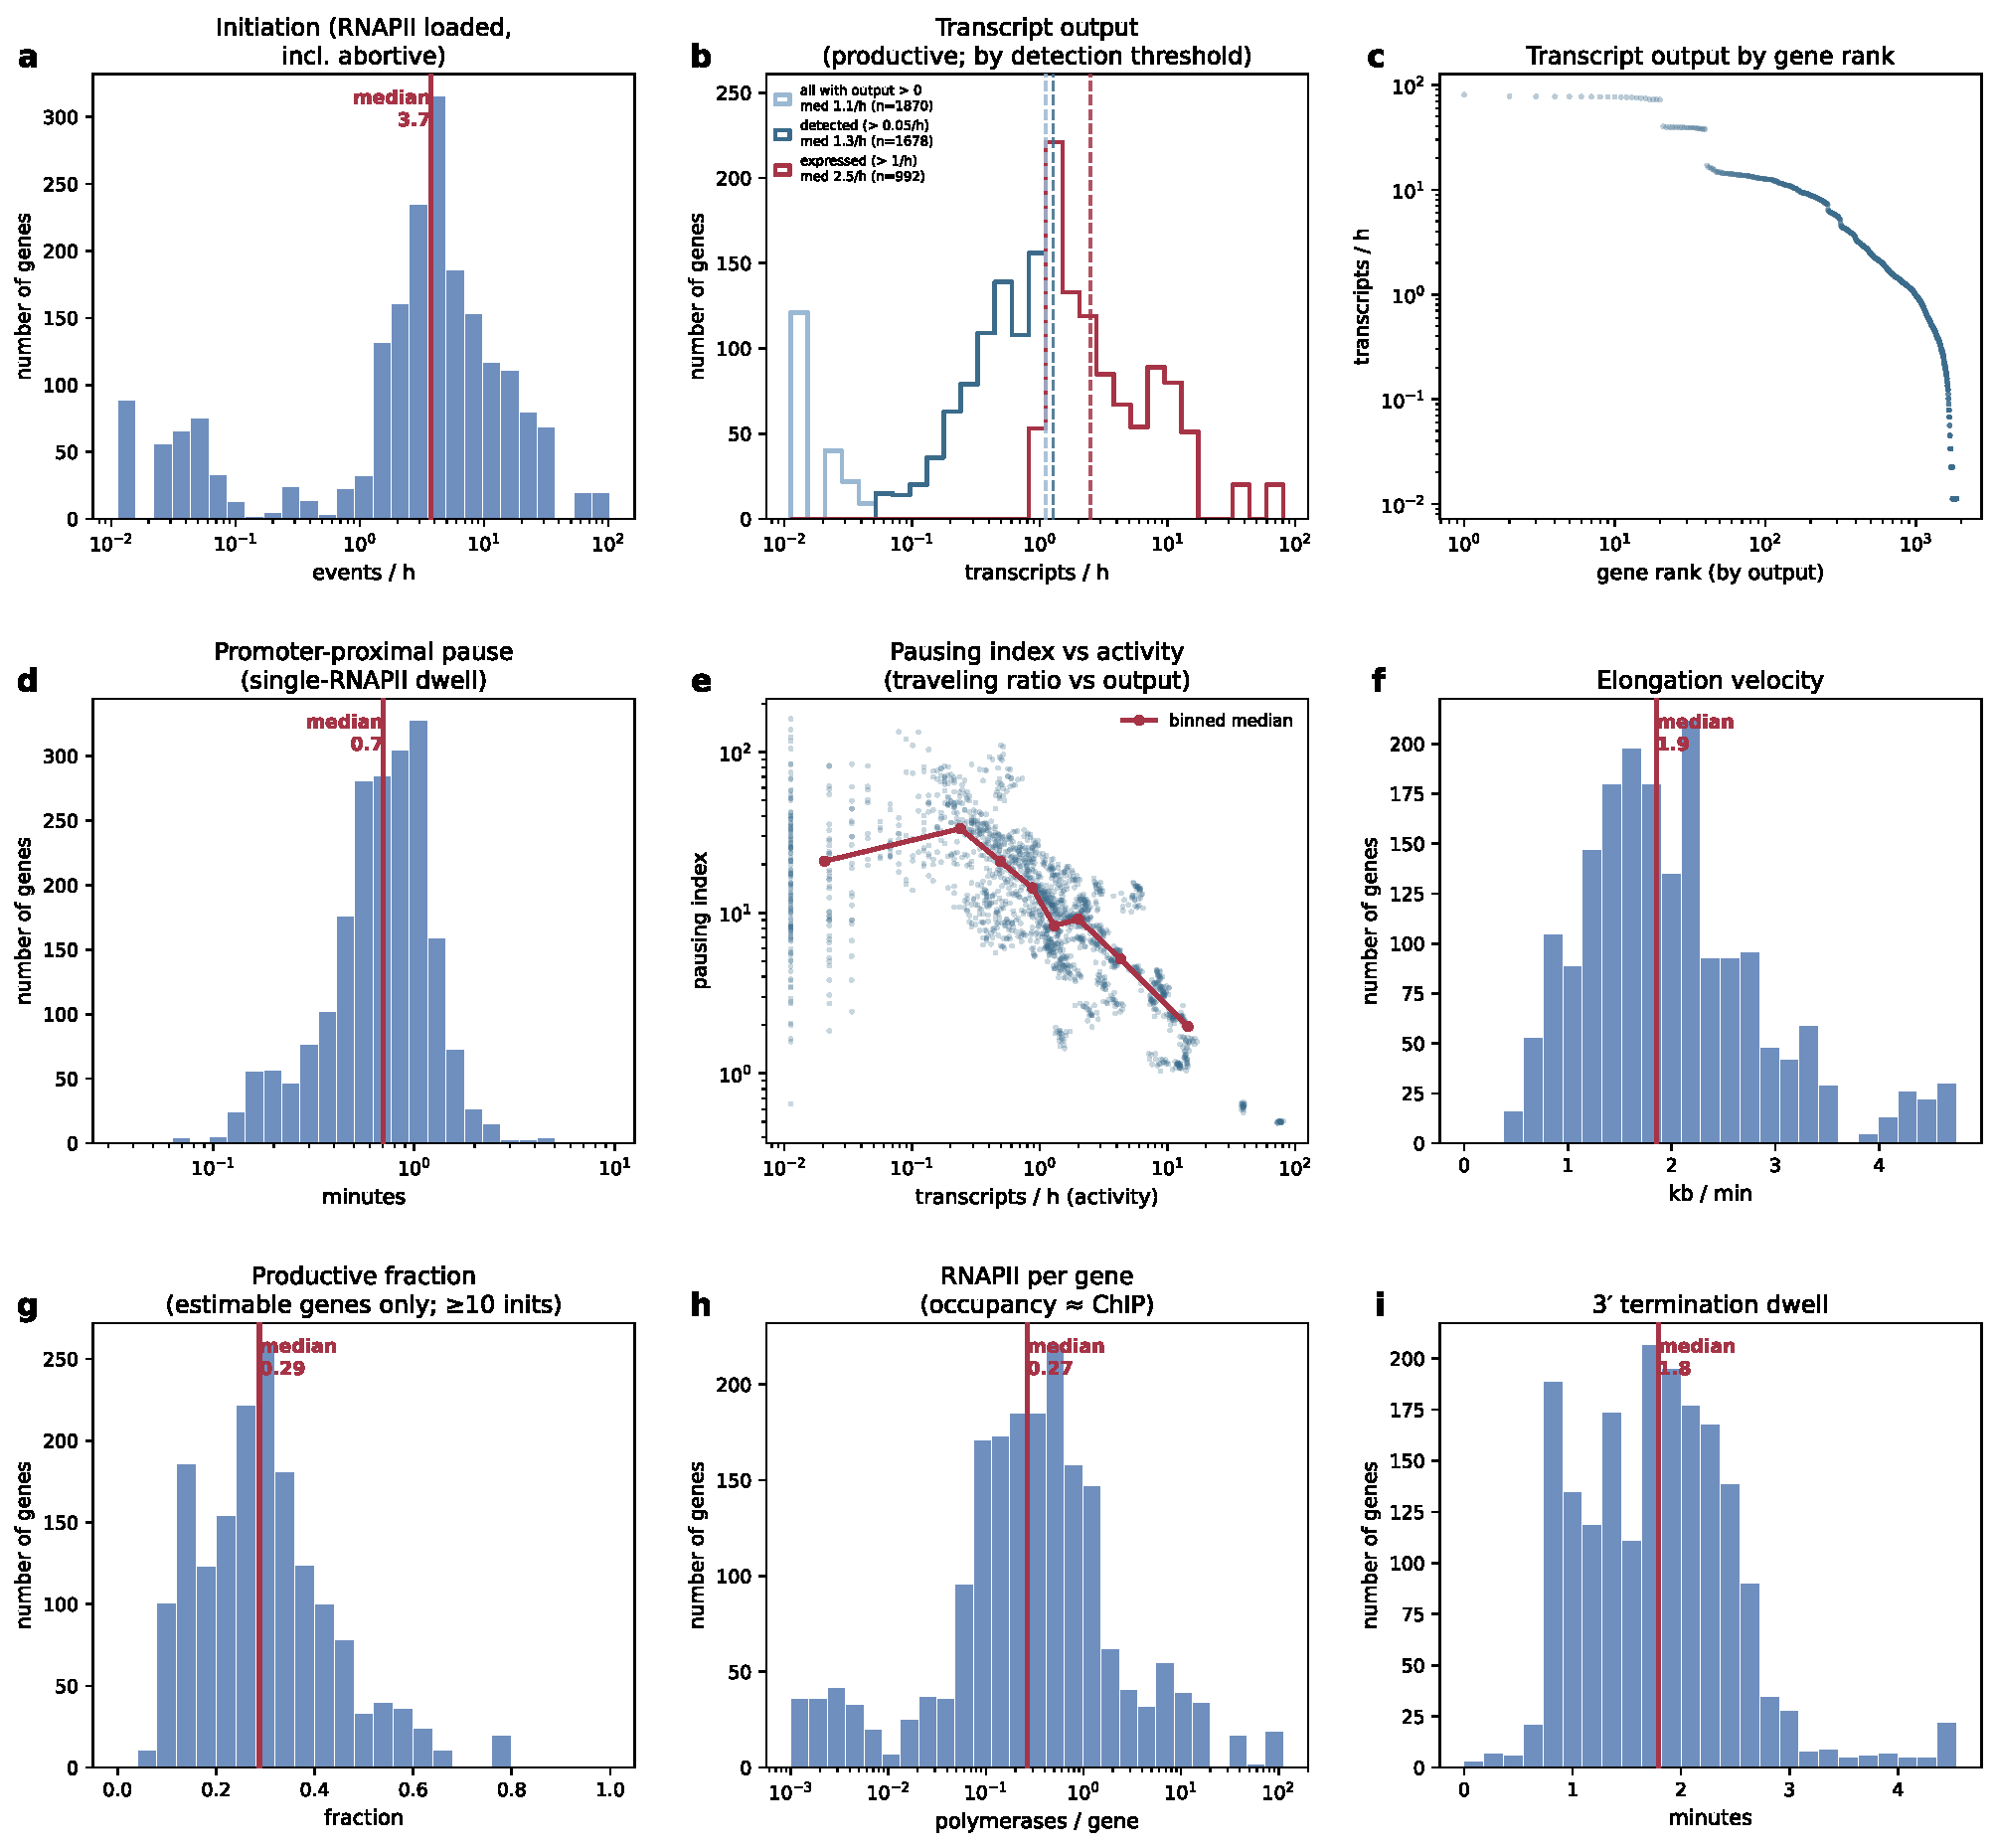
\includegraphics[width=\linewidth]{transcription_distributions_pub.pdf}
\caption{\textbf{Per-allele transcription kinetics across the simulated
allele-instance population.} Distributions over $n=2{,}440$ allele-instances $=$ 122
loci (genes) in the modeled region $\times$ 20 replicate chains; red line, model
median. \textbf{(a)}~Initiation rate (RNAPII loading, including the $\sim$70--80\% that
prematurely terminate at the pause). \textbf{(b)}~Productive transcript output (RNAPII
reaching the 3$'$ end), as nested step histograms at several detection thresholds
(output $>$0, $>$0.05~h$^{-1}$, $>$1~h$^{-1}$), each with its own dashed median, so the
``expressed median'' is cutoff-dependent. \textbf{(c)}~Transcript output by gene rank
(log--log). \textbf{(d)}~Single-polymerase promoter-proximal pause dwell.
\textbf{(e)}~Pausing index versus productive output (log--log) with the binned-median
trend (red); highly expressed genes show a lower pausing index. \textbf{(f)}~Elongation
velocity. \textbf{(g)}~Productive fraction, shown only for genes with $\ge$10
initiations (where the ratio is estimable); genes with fewer (low-confidence) or zero
(undefined) initiations are tallied separately, not plotted as a spike at zero.
\textbf{(h)}~RNAPII occupancy per gene. \textbf{(i)}~3$'$ termination dwell.
Heavy-tailed metrics use a logarithmic axis.}
\label{fig:txn}
\end{figure}

A paused polymerase resolved in one of two competing ways: it either escaped into
productive elongation or terminated prematurely and was lost. The fraction that escaped
--- the productive fraction --- was a per-gene quantity set near the $\approx$0.2
inferred for mammalian promoters, where roughly 80\% of promoter-proximally paused
Pol~II terminate prematurely (Zimmer et al., 2021, by single-molecule STL-seq in human
and \emph{Drosophila} cells; consistent with the rapid turnover of promoter-paused
Pol~II seen by live imaging, Steurer et al., 2018). We made the productive fraction
increase with activity --- lowest at quiet genes ($\approx$0.14) and highest at the
most active genes ($\approx$0.47), reflecting the reduced premature termination of
strongly transcribed promoters --- giving a population median of $\approx$0.29.

The model has a single pause-duration input: the \emph{single-polymerase pause dwell},
the real time one polymerase stays paused before it escapes or terminates. We pinned its
median to $\approx$42~s, the mean promoter-proximal residence time measured by live-cell
imaging of endogenous Pol~II in human cells (Steurer et al., 2018), and anti-correlated
it with activity so that the most active genes cleared the pause fastest ($\approx$25~s)
and poised genes paused longer. The longer, multi-minute \emph{apparent} pause durations
reported by genomic decay-rate measurements (a $\approx$7~min mean in mouse ES cells,
Jonkers et al., 2014; a $\approx$2--30~min range across studies, Core \& Adelman, 2019)
are \emph{not} a second input: they are what that same paused state reads as when pause
occupancy is divided by the much lower productive output (because most paused
polymerases terminate prematurely, as above). Measured that way, the model's
apparent pause was $\approx$2.6~min --- so one $\approx$42~s single-molecule dwell
reproduces both the live-imaging and the decay-rate conventions.

We drew per-gene activity from a heavy-tailed, power-law distribution spanning two to
three orders of magnitude, approximating the broad, continuous spread of transcription
rates across genes. Each gene's polymerase-loading propensity combined its pause-escape
probability, a weak inverse power of its domain length (so genes in shorter, more active
domains recruited more often) and a power-law scatter term, renormalised so that the
geometric-mean loading of the expressed set met a fixed target and then scaled by an
absolute per-class factor:
%
\begin{equation}
r_i = r_0\,\frac{\rho_i}{\big(\prod_{j\in\mathcal{E}}\rho_j\big)^{1/|\mathcal{E}|}}\;c_{c(i)},
\qquad
\rho_i = p^{\mathrm{esc}}_i\left(\frac{\tilde L}{L_{T(i)}}\right)^{\eta}\pi_i,
\quad \pi_i\sim\mathrm{PowerLaw}(\gamma),
\end{equation}
%
where $r_i$ is gene $i$'s loading propensity, $r_0$ the target geometric-mean loading
over the expressed set $\mathcal{E}$, $c_{c(i)}$ its regulatory-class multiplier,
$p^{\mathrm{esc}}_i$ its pause-escape probability, $L_{T(i)}$ its domain length, $\tilde
L$ the median gene-hosting domain length, $\eta\approx0.2$ a weak size exponent and
$\pi_i$ a power-law (Zipf) scatter term (exponent $\gamma\approx2.4$). A defined
fraction of the regulated-class genes was held effectively silent; rather than a hard
zero, silent genes received a graded, near-zero loading spanning deep-silent (no
initiation over the trajectory) up to a low basal/leaky level, so that the
silent-to-expressed transition formed a continuum rather than a spike-and-gap, as in
real transcriptomes.

Escaped polymerases translocated in their transcriptional direction at a gene-specific
velocity drawn around a 2.1~kb\,min$^{-1}$ anchor (0.035~kb\,s$^{-1}$; per-gene range
$\approx$0.5--6~kb\,min$^{-1}$), within the 1.3--4.3~kb\,min$^{-1}$ reported for
mammalian Pol~II in vivo (Guo \& Price, 2013) and bracketing the 0.5--4~kb\,min$^{-1}$
measured genome-wide in mouse ES cells (Jonkers et al., 2014); steric exclusion among
co-transcribing polymerases reduced the realised median to $\approx$1.9~kb\,min$^{-1}$,
close to the rate assumed in genome-wide initiation inference (Zhao et al., 2023).
Multiple polymerases could co-occupy a gene subject to steric exclusion, so
inter-polymerase spacing emerged self-consistently. On reaching the 3$'$ end a
polymerase decelerated and dwelt over the termination zone for $\approx$1.8~min before
release; this dwell represents the multi-kilobase termination window downstream of the
poly(A) site (Fong et al., 2015), across which Pol~II decelerates from $>$2 to
$<$1~kb\,min$^{-1}$ (Cortazar et al., 2019), and the terminating polymerase is the
proximate cause of cohesin accumulation at 3$'$ ends. For regulated-class genes, pause
escape was permitted only while the gene's promoter and a cognate enhancer were
co-contained within a single cohesin loop, gating a subset of productive initiation on
the instantaneous loop-extrusion state and reproducing the cohesin-dependence of
enhancer-driven activation established for Mediator--cohesin looping (Kagey et al.,
2010) and enhancer--promoter communication (Narita et al., 2025).

Across the population (122 genes $\times$ 20 replicate chains $=$ 2{,}440
allele-instances; Fig.~\ref{fig:txn}), these kinetics reproduced genome-scale
transcription statistics. About 69\% of alleles were detectably transcribed (productive
output $>$0.05~transcripts\,h$^{-1}$); the rest formed a continuum from deep-silent to
low basal output, with $\approx$23\% producing no completed transcript and $\approx$17\% never initiating at all. The typical
detected allele made $\approx$1.3~transcripts\,h$^{-1}$ ($\approx$2.5 per diploid gene),
close to the $\approx$2~mRNA\,h$^{-1}$ average synthesis rate measured genome-wide in
mammalian cells (Schwanh\"ausser et al., 2011), and per-gene output was heavy-tailed,
with a thin active tail reaching tens of transcripts\,h$^{-1}$. Promoter-proximal
pausing was prevalent, with a median pausing (traveling-ratio) index of $\approx$6 over
expressed genes, in line with the widespread pausing of mammalian genes (Day et al.,
2016). The modeled locus is gene-rich and transcriptionally active --- more active than
the genome-wide median --- yet its global output stays well below the
\emph{hypertranscription} of cancer cells, which raise genome-wide RNA output roughly
twofold (a mean $\approx$2.2-fold increase in total RNA output across human cancers,
up to $\approx$3.5-fold in aggressive subtypes; Zatzman et al., 2022 --- a relative,
genome-wide ratio, not a per-allele rate), an amplification of the existing expression
program associated with elevated MYC (Lin et al., 2012; though MYC's direct action is
substantially gene-selective, Sab\`o et al., 2014; Walz et al., 2014). The hottest
model genes accordingly fall short of cancer-line single-gene maxima: our top alleles
reach $\approx$1.3 productive events\,min$^{-1}$ \emph{per allele} ($\approx$2.6 per
diploid gene), whereas a strongly induced gene such as HSPA1A reaches $\approx$87
events\,min$^{-1}$ \emph{per cell} upon heat-shock induction in the hyper-transcribing
human line K562 (Gressel et al., 2019). (All per-gene rates we report for the model are
per allele; a diploid gene is twice that.) Our parameters thus describe an active,
non-malignant locus, and a single loading-rate constant tunes the overall level between
these regimes.

% =====================================================================
\section{RNA polymerase II -- cohesin interactions}

We treated an engaged polymerase as a permeable, motile barrier to extrusion
(Banigan et al., 2023), resolving two encounter geometries. When a cohesin subunit
attempted to step onto a polymerase-occupied site it succeeded only stochastically;
the mean transit time past a transcriptionally engaged (paused, elongating or
terminating) polymerase was $\approx$100~s, the bypass rate ($\approx$0.01~s$^{-1}$)
that best reproduces transcription's effect on contact maps (Banigan et al., 2023).
Two quantities define this barrier, the per-step probability that a subunit is
blocked rather than passing, and the velocity margin that makes the barrier directional:
%
\begin{equation}
p_{\mathrm{block}} = e^{-\Delta t/\tau_{\mathrm{bypass}}},
\qquad
\tau_{\mathrm{bypass}}^{\mathrm{engaged}} \approx 100\ \mathrm{s}\
(p_{\mathrm{block}}\approx0.98),
\qquad
\frac{v_{\mathrm{sub}}}{v_{\mathrm{elong}}} \approx 3.6.
\end{equation}
%
A merely pre-initiation polymerase was $\approx$8-fold more permeable
($\tau_{\mathrm{bypass}}\approx 12$~s). We did not accelerate the turnover of a
cohesin held against a polymerase: its unbinding rate remained the baseline value.
The framework permits an accelerated cohesin-eviction regime (the analogue of the
Wapl-mediated release that frees active genes of cohesin in vivo; Busslinger et al.,
2017), but a short eviction lifetime depletes rather than accumulates cohesin at
active genes, so we left it inactive: the gene-body and 3$'$ enrichment arose
entirely from the moving-barrier relocation described next.

Reciprocally, an elongating polymerase that collided with a cohesin subunit most
often relocated it (displacing the subunit ahead and translating the loop along
the gene) when the two converged head-on, and more often arrested itself when
co-directional; non-elongating polymerases did not relocate cohesin. This rectified
interaction drove cohesin accumulation at and beyond 3$'$ ends and the formation of
cohesin islands between convergent genes (Banigan et al., 2023; Busslinger et al.,
2017). In the polymerase-free configurations (the transcription-off control and the
repair experiments) these interactions were absent and cohesin responded only to
boundaries, other cohesins and lesions.

% =====================================================================
\section{Lesions}

We represented ultraviolet photoproducts, predominantly cyclobutane pyrimidine
dimers and 6-4 photoproducts, the substrates of nucleotide-excision repair (NER),
as damaged lattice sites that were induced at a controlled density, progressed
through a two-stage repair trajectory and were excised. We maintained the
population homeostatically at a fixed target $M$ equal to the lattice length divided
by the chosen lesion spacing $s$ (the experimental analogue of UV dose; below),
%
\begin{equation}
M = \left\lfloor \frac{L_{\mathrm{tot}}}{s} \right\rfloor.
\end{equation}
%
On each step we advanced existing lesions, deleted those that completed repair, and
spawned new lesions until the target was restored, so that the steady-state damage
burden was constant while individual lesions turned over; on the first step the
population was seeded directly by the spawner.

We spawned each new lesion by weighted random sampling of lattice sites. Every site
$i$ carried a weight equal to the length of its host domain raised to a negative
tunable power, and its induction probability was that weight normalised over the
lattice,
%
\begin{equation}
P(\text{induce at site } i) = \frac{L_{T(i)}^{-\alpha}}{\sum_{j} L_{T(j)}^{-\alpha}},
\qquad \alpha = 1,
\end{equation}
%
where $L_{T(i)}$ is the length of the domain containing site $i$ and $\alpha$ the
steepness of the size bias (the configuration key \texttt{lesion\_tad\_size\_exponent};
here $\alpha=1$). The per-tick deficit was drawn in batches and rejection-sampled
(sites already carrying a lesion were rejected and redrawn), and because the weights
are normalised, any reference length cancels and only the \emph{relative} domain
lengths enter. The exponent sets how the fixed damage budget $M$ partitions across
domains: a domain of length $L$ spans $L$ sites, each weighted $L^{-\alpha}$, so its
expected share of lesions scales as $L\cdot L^{-\alpha}=L^{1-\alpha}$. At $\alpha=0$
induction is spatially uniform, with a domain's lesion count growing in proportion to its
length, at constant per-kilobase density; at $\alpha=1$, the value we used, every
domain accrues in expectation a similar \emph{number} of lesions regardless of size,
so the per-kilobase damage density scales as $1/L$ and shorter domains are
proportionally more heavily damaged; at $\alpha>1$ shorter domains would carry more
damage even in absolute count. Every new lesion entered in the pre-repair state. The
same inverse-domain-length bias, through the exponent $\beta$ of Eq.~10, also speeds
recognition and repair in shorter domains, so chromatin context shapes both ends of
the lesion life cycle.

Lesion spacing is the experimental analogue of UV dose; our wet-lab experiments used
20~J\,m$^{-2}$ UVC, which generates $\approx$1 photolesion (CPD and 6-4PP combined) per
15~kb of single-stranded DNA (Quinet et al., 2016, after Andrade-Lima et al., 2015),
i.e.\ $\approx$1 per 7.5~kb of duplex DNA (derived from the per-strand value). With the assumption that UV photoproduct yield is approximately linear in dose over this range,
the equivalent dose of any spacing follows from this anchor by inverse proportionality:
%
\begin{equation}
D \approx D_0\,\frac{s_0}{s} \approx \frac{150\ \mathrm{kb\cdot J\,m^{-2}}}{s},
\qquad (D_0,\,s_0) = (20\ \mathrm{J\,m^{-2}},\ 7.5\ \mathrm{kb}).
\end{equation}
%
with $D$ the equivalent UVC dose, $s$ the lesion spacing (in kb) and $(D_0,\,s_0)$ the
20~J\,m$^{-2}$ anchor. After irradiation, nucleotide-excision repair clears lesions over
hours to days, lowering their genomic density. We modelled this time-course as a sweep of
the spacing from $\approx$7~kb (the fresh $\approx$22~J\,m$^{-2}$ burden) up to $\approx$100~kb
(largely repaired), running each spacing as an independent steady-state simulation, a
snapshot of the lesion burden at one post-exposure time (Table~2).

\medskip
\noindent\textbf{Table 2. Lesion-density calibration and repair-time sweep.} Top row:
duplex-DNA photoproduct yield at the 20~J\,m$^{-2}$ experimental dose (the initial burden).
Bottom row: the swept lesion-spacing range, modelling the post-exposure repair time-course;
Eq.~8 gives the equivalent dose of each density.

\medskip
\noindent\begin{tabularx}{\linewidth}{@{}>{\raggedright\arraybackslash}p{3.6cm} >{\raggedright\arraybackslash}p{2.6cm} >{\raggedright\arraybackslash}p{2.8cm} Y@{}}
\toprule
Lesion spacing (duplex DNA) & Lesion density & UVC dose & Basis \\
\midrule
1 per $\approx$7.5~kb & 133 lesions~Mb$^{-1}$ & 20~J\,m$^{-2}$ & Quinet et al., 2016 (1 per 15~kb / strand); Andrade-Lima et al., 2015 \\
1 per 7--100~kb (swept) & 143--10 lesions~Mb$^{-1}$ & & this study (repair time-course via decreasing densities over independent simulations) \\
\bottomrule
\end{tabularx}

\medskip
We typed each lesion at the moment of induction. A lesion falling within a gene body
was assigned to the transcription-coupled pathway (TC-NER; ``Type A'') with a fixed
probability (the TC-NER fraction) and otherwise to the global-genome pathway
(GG-NER; ``Type B'');
every lesion outside a gene body was GG-NER,
%
\begin{equation}
P(\text{TC-NER}\mid i) =
\begin{cases}
f_A, & i \in \text{gene body},\\[2pt]
0, & \text{otherwise},
\end{cases}
\qquad f_A \le \tfrac{1}{2},
\end{equation}
%
the complement being GG-NER. TC-NER lesions represent damage on the transcribed
strand of an active gene, where an elongating polymerase arrests: the stalled
polymerase both designates the lesion for rapid, dedicated repair and constitutes
the physical obstruction, and these lesions are the model's representation of
polymerase-stalling events. GG-NER lesions (intergenic damage and the
non-transcribed-strand or non-stalling remainder within genes) are recognised by
the genome-wide surveillance pathway. We treated the TC-NER fraction as a swept
quantity; because only the transcribed strand of an active gene yields a stalling
event and the slowly excised cyclobutane dimers dominate persistent stalls, its
physical ceiling is one-half and its realistic value $\approx$one-quarter. In a
control in which global-genome repair was disabled, the transcription-coupled
lesions were instead held at their unchanged expected count and drawn only from
gene-body sites, so that the TC-NER burden matched the full-repair run rather than
being inflated.

Each lesion then followed a two-state, memoryless repair trajectory with no internal
countdown, exactly as for cohesin turnover. At every step a pre-repair lesion
advanced to the repair state, and a repair-state lesion was excised and removed,
with per-step probabilities
%
\begin{equation}
p_{\mathrm{PRE}\to\mathrm{REP}}
= \min\!\Big(1,\ \tfrac{\Delta t}{\tau_{\mathrm{pre}}}\,\mu_i\Big),
\qquad
p_{\mathrm{REP}\to\varnothing}
= \min\!\Big(1,\ \tfrac{\Delta t}{\tau_{\mathrm{rep}}}\,\mu_i\Big),
\qquad
\mu_i = \Big(\frac{\bar L}{L_{T(i)}}\Big)^{\beta},
\end{equation}
%
with mean pre-repair time $\tau_{\mathrm{pre}}\approx40$~min, mean repair time
$\tau_{\mathrm{rep}}\approx6$~min, $\bar L$ the mean domain length and $\beta=1$. The
multiplier $\mu_i$ exceeds one in shorter-than-average domains and is below one in
longer ones (the per-step probability itself being capped at one, via the $\min$), so
lesions in shorter domains were recognised and repaired faster and those in longer
domains more slowly, the same chromatin-context dependence acting on repair as on
induction. The stage durations
and the lesion density jointly set the steady-state probability that any site
carries an obstructing lesion.

% =====================================================================
\section{Lesion -- cohesin interactions}

In the lesion experiments transcription was switched off and no transcribing
polymerases were simulated; instead, a transcription-coupled (Type~A) lesion in its
pre-repair stage stood in for the elongating polymerase stalled at the damage,
supplying the same cohesin obstruction at the same genomic site. We adopted this static
stand-in rather than dynamically simulating a polymerase arresting at a lesion, being
displaced during repair and re-initiating afterwards, because the kinetics of
transcription recovery after UV damage --- the timing of polymerase removal,
repair-coupled restart and re-initiation --- are not characterised well enough to
parameterise a dynamic transcription--lesion coupling. The lesion field therefore
represents the steady-state obstruction that stalled polymerases and bound repair
machinery present to loop extrusion, without committing to an under-determined recovery
timescale.

A lesion's effect on cohesin was conditioned on its repair stage and pathway. A
lesion in the active repair stage, of either pathway, arrested an incident cohesin
subunit with high per-step probability ($\approx$0.993; bypass $\approx$0.007 per step), representing the bound
repair machinery occluding the duplex. A TC-NER lesion in the pre-repair stage
arrested cohesin only in the polymerase-free configurations, where it substituted
for the stalled polymerase that would otherwise provide the obstruction; when
polymerases were simulated the block was supplied by the genuine arrested polymerase
(Section~5) and the lesion did not independently arrest cohesin in this stage,
avoiding double counting. A GG-NER lesion in the pre-repair stage was
transparent to cohesin, there being no occluding complex before machinery assembly.
An arrested subunit failed to advance for as long as the lesion persisted and was
released when the lesion completed repair or the complex turned over at the baseline
rate (no accelerated eviction, as for a polymerase barrier; Section~5). Because only
the leading subunit was tested per step, a complex continued extruding on its
unobstructed side while one subunit was arrested, the mechanism by which a field
of lesions reshapes, rather than abolishes, the distribution of cohesin loops.

% =====================================================================
\section{Simulation pipeline}

All results were produced by a single driver, executing the configurations and
analyses in a fixed sequence under the calibration of Section~1 (250~bp per site, 2~s
per step; $\approx$22~h equilibration and $\approx$89~h production per run).

We generated a 10-Mb locus (122 genes across 10 domains) and instantiated it as
twenty independent replicates, producing two matched configurations: a
transcription-on baseline with active polymerases, and a transcription-off control
with identical genes, domains and boundaries but no polymerases, whose contrast
isolates the effect of transcription at fixed architecture. In this comparison,
transcription shortened the mean cohesin loop (from $\approx$248 to $\approx$216~kb),
enriched cohesin within gene bodies ($\approx$1.1-fold), and depleted it from CTCF
boundaries ($\approx$1.3-fold) and from domain-spanning corner dots ($\approx$4.4-fold) relative
to the transcription-off control (all $P<0.001$ over the twenty replicates), the
moving-barrier signature of transcription on chromosome folding (Banigan et al., 2023).
We simulated both and,
across the two conditions, compared a panel of cohesin-distribution metrics (defined in
Table~3): the mean loop length, cohesin occupancy at gene bodies and at CTCF boundaries,
boundary-pass (read-through) events, boundary-crossing stripes and the corner-dot frequency.
We swept boundary arrest probabilities
up to $\approx$6-fold to map the dependence of the cohesin distribution on insulation
strength. In the polymerase-free condition we introduced lesions and
performed three two-dimensional sweeps: the TC-NER (polymerase-stalling) fraction
against lesion density; the per-step blocking probability against density; and
the recognition and repair timescales against density. In these experiments the
pre-repair stage lasted $\approx$40~min, the repair stage $\approx$6~min, the
per-step block probability was $\approx$0.993, and boundaries were at the
strengthened (3.25-fold) setting. Finally, keeping transcription active in both the swept grid
and the reference, we mapped the cohesin-distribution metrics over a two-dimensional grid of
cohesin residence times, the
free cohesin lifetime against the CTCF-captured (WAPL-protected) lifetime, each scanned from
one-eighth to sixfold of its calibrated value and reported as fold changes relative to the
transcription-on baseline, to separate the contributions of extrusion processivity and CTCF stabilisation
to loop length and boundary occupancy.

\medskip
\noindent\textbf{Table 3. Cohesin-distribution metrics.} All are computed from the
one-dimensional cohesin trajectories (one complex $=$ two subunits; 1~site $=$ 250~bp; 2~s per
sampled frame) and averaged over all sampled frames and the twenty replicates; a site counts
as a CTCF anchor when it lies in the oriented capture window of a domain boundary.

\medskip
\noindent\begin{tabularx}{\linewidth}{@{}>{\raggedright\arraybackslash}p{3.3cm} Y@{}}
\toprule
Metric & Definition \\
\midrule
Mean loop length & The size of the chromatin loop held by a cohesin complex (the genomic
distance between its two subunits), averaged over every complex and every sampled frame (kb).
It reports the typical extruded loop size. \\
Cohesin at gene bodies & The mean cohesin occupancy of gene bodies: every cohesin subunit lying
inside a gene body is counted, then divided by the number of gene-body sites and the number of
sampled frames. A high value reflects cohesin enrichment within transcribed genes. \\
Cohesin at CTCF boundaries & The same occupancy measure evaluated at CTCF-anchor sites (mean
subunits per anchor site per frame). A high value reflects cohesin accumulation (parking)
against convergent CTCF boundaries. \\
Boundary-pass events & How often extrusion reads through a boundary instead of being arrested:
for each internal boundary, the rate of single-site subunit steps that cross it, per boundary per
time step (genuine one-site moves only; complexes that unbind and reload elsewhere are excluded).
It measures boundary permeability. \\
Boundary-crossing stripe & A one-sided loop that straddles a boundary: one subunit stays captured
at a CTCF anchor while the other extrudes past a domain boundary, leaving the loop with a single
anchored end (counted per boundary per frame). This asymmetric configuration produces an
architectural stripe on a contact map; by contrast, a corner dot has both subunits anchored. \\
Corner dot & A loop that pins an entire domain: one subunit captured at the domain's left anchor
and the other at its right anchor, bridging it end to end (counted per internal domain per frame).
It is the one-dimensional counterpart of the focal corner dot seen at a domain's apex on a
contact map. \\
\bottomrule
\end{tabularx}

% =====================================================================
\section*{References}
\addcontentsline{toc}{section}{References}
\begin{enumerate}\setlength{\itemsep}{2pt}
\item Dixon, J. R. et al. Topological domains in mammalian genomes identified by
analysis of chromatin interactions. \textit{Nature} 485, 376--380 (2012).
\item Rao, S. S. P. et al. A 3D map of the human genome at kilobase resolution
reveals principles of chromatin looping. \textit{Cell} 159, 1665--1680 (2014).
\item Kagey, M. H. et al. Mediator and cohesin connect gene expression and
chromatin architecture. \textit{Nature} 467, 430--435 (2010).
\item Busslinger, G. A. et al. Cohesin is positioned in mammalian genomes by
transcription, CTCF and Wapl. \textit{Nature} 544, 503--507 (2017).
\item Davidson, I. F. et al. DNA loop extrusion by human cohesin. \textit{Science}
366, 1338--1345 (2019).
\item Kim, Y., Shi, Z., Zhang, H., Finkelstein, I. J. \& Yu, H. Human cohesin
compacts DNA by loop extrusion. \textit{Science} 366, 1345--1349 (2019).
\item Gabriele, M. et al. Dynamics of CTCF- and cohesin-mediated chromatin looping
revealed by live-cell imaging. \textit{Science} 376, 496--501 (2022).
\item Hansen, A. S., Pustova, I., Cattoglio, C., Tjian, R. \& Darzacq, X. CTCF and
cohesin regulate chromatin loop stability with distinct dynamics. \textit{eLife} 6,
e25776 (2017).
\item Yang, J. H. \& Hansen, A. S. Enhancer selectivity in space and time: from
enhancer--promoter interactions to promoter activation. \textit{Nat. Rev. Mol. Cell
Biol.} 25, 574--591 (2024).
\item Banigan, E. J. et al. Transcription shapes 3D chromatin organization by
interacting with loop extrusion. \textit{Proc. Natl Acad. Sci. USA} 120, e2210480120
(2023).
\item Banigan, E. J., van den Berg, A. A., Brand\~{a}o, H. B., Marko, J. F. \&
Mirny, L. A. Chromosome organization by one-sided and two-sided loop extrusion.
\textit{eLife} 9, e53558 (2020).
\item Fudenberg, G. et al. Formation of chromosomal domains by loop extrusion.
\textit{Cell Rep.} 15, 2038--2049 (2016).
\item Imakaev, M., Goloborodko, A. \& Brand\~{a}o, H. B. mirnylab/polychrom.
\textit{Zenodo} \url{https://doi.org/10.5281/zenodo.3579473} (2019).
\item Gressel, S., Schwalb, B. \& Cramer, P. The pause-initiation limit restricts
transcription activation in human cells. \textit{Nat. Commun.} 10, 3603 (2019).
\item Zhao, Y., Liu, L., Hassett, R. \& Siepel, A. Model-based characterization of
the equilibrium dynamics of transcription initiation and promoter-proximal pausing
in human cells. \textit{Nucleic Acids Res.} 51, e106 (2023).
\item Jonkers, I., Kwak, H. \& Lis, J. T. Genome-wide dynamics of Pol II elongation and
its interplay with promoter proximal pausing, chromatin, and exons. \textit{eLife} 3,
e02407 (2014).
\item Steurer, B. et al. Live-cell analysis of endogenous GFP-RPB1 uncovers rapid turnover
of initiating and promoter-paused RNA polymerase II. \textit{Proc. Natl Acad. Sci. USA}
115, E4368--E4376 (2018).
\item Core, L. \& Adelman, K. Promoter-proximal pausing of RNA polymerase II: a nexus
of gene regulation. \textit{Genes Dev.} 33, 960--982 (2019).
\item Guo, J. \& Price, D. H. RNA polymerase II transcription elongation control.
\textit{Chem. Rev.} 113, 8583--8603 (2013).
\item Fong, N. et al. Effects of transcription elongation rate and Xrn2 exonuclease
activity on RNA polymerase II termination. \textit{Mol. Cell} 60, 256--267 (2015).
\item Cortazar, M. A. et al. Control of RNA Pol II speed by PNUTS-PP1 and Spt5
dephosphorylation facilitates termination by a ``sitting duck torpedo'' mechanism.
\textit{Mol. Cell} 76, 896--908 (2019).
\item Zimmer, J. T., Rosa-Mercado, N. A., Canzio, D., Steitz, J. A. \& Simon, M. D.
STL-seq reveals pause-release and termination kinetics for promoter-proximal paused
RNA polymerase II transcripts. \textit{Mol. Cell} 81, 4398--4412 (2021).
\item Schwanh\"ausser, B. et al. Global quantification of mammalian gene expression
control. \textit{Nature} 473, 337--342 (2011).
\item Day, D. S. et al. Comprehensive analysis of promoter-proximal RNA polymerase II
pausing across mammalian cell types. \textit{Genome Biol.} 17, 120 (2016).
\item Narita, T. et al. Disentangling the architectural and non-architectural
functions of CTCF and cohesin in gene regulation. \textit{Nat. Genet.} 57,
3137--3151 (2025).
\item Lin, C. Y. et al. Transcriptional amplification in tumor cells with elevated
c-Myc. \textit{Cell} 151, 56--67 (2012).
\item Sab\`o, A. et al. Selective transcriptional regulation by Myc in cellular growth
control and lymphomagenesis. \textit{Nature} 511, 488--492 (2014).
\item Walz, S. et al. Activation and repression by oncogenic MYC shape tumour-specific
gene expression profiles. \textit{Nature} 511, 483--487 (2014).
\item Zatzman, M. et al. Widespread hypertranscription in aggressive human cancers.
\textit{Sci. Adv.} 8, eabn0238 (2022).
\item Quinet, A. et al. Translesion synthesis mechanisms depend on the nature of DNA
damage in UV-irradiated human cells. \textit{Nucleic Acids Res.} 44, 5717--5731 (2016).
\item Andrade-Lima, L. C., Veloso, A., Paulsen, M. T., Menck, C. F. M. \& Ljungman, M.
DNA repair and recovery of RNA synthesis following exposure to ultraviolet light are
delayed in long genes. \textit{Nucleic Acids Res.} 43, 2744--2756 (2015).
\end{enumerate}

\end{document}
